\newpage
\section{Apprendimento per rinforzo}

L'apprendimento che deriva dall'\textbf{interazione} con un ambiente è una
forma di intelligenza molto comune, la più nota, semplice e intuitiva.

\begin{figure}[H]
\caption{Scenario descrittivo dell'apprendimento per rinforzo}
\centering
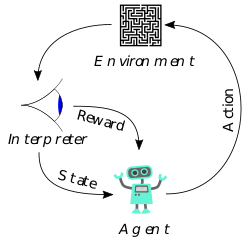
\includegraphics[width=0.5\textwidth]{learning}
\end{figure}

L'apprendimento per rinforzo è guidato da un \textbf{obiettivo}, che viene
usato per stabilire se un'interazione con l'ambiente è positiva o negativa.

L'apprendimento per rinforzo consiste nel sapere quale azione intraprendere in
una data situazione, così da massimizzare la \textbf{ricompensa} (di solito
espressa in forma numerica).

Chi apprende attraverso questo meccanismo deve scoprire quali azioni producono
la maggior ricompensa provandole.

La ricerca ``prova, sbaglia, impara'' e la ``ricompensa con slack'' sono due
importanti concetti.\\

Un agente che apprende deve saper riconoscere lo stato dell'ambiente in cui si trova
e interagire con esso in modo tale da cambiarlo. Deve anche sapere qual è
l'obiettivo da raggiungere.

L'apprendimento per rinforzo è diverso sia dall'apprendimento supervisionato (non
dispone di esempi passati che possano dirgli quale sia la cosa giusta da fare, deve
essere in grado di apprendere da se stesso) che dall'apprendimento non supervisionato
(non deve tentare di trovare patterns o strutture in dati sconosciuti) quello che
deve fare, principalmente, è tentare di massimizzare la ricompensa.

Un agente che apprende deve \textbf{sfruttare} ciò che ha imparato in passato per ottenere una
ricompensa, ma deve anche \textbf{esplorare} nuove azioni per sceglierne di migliori in futuro.

Questo tipo di approccio permette di gestire le \textbf{incertezze} dell'ambiente in
cui l'agente si trova.
